\chapter{熟悉并行编程环境}
\section{实验目的与要求}
\par 熟悉并行编程环境,并行编程的基本法则和方法以及在Linux下使用pthread、OpenMP、MPI的性能优化方法。

\section{实验内容}
\subsection{熟悉Linux下的并行编程环境}
\label{sub:shou_xi_linuxxia_de_bing_xing_bian_cheng_huan_jing_}
\par 首先,需要熟悉Linux下的并行编程环境。并行编程的平台有很多,而广泛使用的有pthread、OpenMP、MPI、CUDA等平台,其中前3种运行在CPU上而第四种则在CPU与GPU上混合运行。下面使用简单的向量加法来说明各个环境的运行机制。

\paragraph{串行的向量加法}
\label{par:chuan_xing_de_xiang_liang_jia_fa_}
\par 令\(\vec{a}, \vec{b}, \vec{c}\)为3个长度为\(n\)的向量,则求\(\vec{c} = \vec{a} + \vec{b}\)的串行过程如下:
\begin{simpleAlgorithm}{串行加法}
    \Procedure{SerialAdd}{$\vec{a}, \vec{b}, \vec{c}, n$}
    \For{$i = 1$ \textbf{to} $n$}
    \State \(c[i] = a[i] + b[i]\)
    \EndFor
    \EndProcedure
\end{simpleAlgorithm}

\par 这样,\(c[i] = a[i] + b[i]\) 需要被执行\(n\)次,设每次执行的平均时间为\(t\)则共需至少\(n\times t\)的时间。当\(n\) 非常大时,此算法需要的时间则较长,而并行算法则是使执行这些加法的时间有不同程度的重叠,从而减少程序执行所需要的总时间。

\paragraph{使用pthread执行向量加法}
\label{par:shi_yong_pthreadzhi_xing_xiang_liang_jia_fa_}
\par Pthread(POSIX Threads),是POSIX的线程标准,定义了创建和操纵线程的一套API。一般用于Unix-like POSIX 系统,如Linux、 Solaris。其中包含了以下的功能:
\begin{enumerate}
    \item 线程管理,例如创建线程,等待(join)线程,查询线程状态等。
    \item 互斥锁(Mutex):创建、摧毁、锁定、解锁、设置属性等操作
    \item 条件变量(Condition Variable):创建、摧毁、等待、通知、设置与查询属性等操作
    \item 使用了互斥锁的线程间的同步管理
\end{enumerate}

\inputCodeSetLanguage{c++}
\par 要使用pthread执行线程加法,需要创建线程,使用多个线程对于不同的分块进行加法运算,最后等待所有的线程完成。创建线程以及等待所有线程完成的一个代码示例如下,使用\lstinline{pthread_create}创建线程,使用\lstinline{pthread_join}等待所有线程完成。\lstinline{pthread_create}世纪上传给\lstinline{sum_array}的参数只有一个,因此如果需要在创建线程时传递多个参数,可以通过class进行参数的打包,也可以使用分配在堆上的变量(如全局变量等)进行传参。

\begin{lstlisting}
for (int i = 0; i < MAX_THREAD; i++)
    pthread_create(&threads[i], NULL, sum_array, (void*)NULL);
for (int i = 0; i < MAX_THREAD; i++)
    pthread_join(threads[i], NULL);
\end{lstlisting}
\par 上述创建以及等待线程的代码时几乎所有使用pthread的程序都需要使用的代码。pthread库中大致有100个函数调用,此处不再详细列举。在后面的实验中可以看到,这些函数是如何紧密配合从而写出高性能的串行代码的。

\paragraph{使用OpenMP执行向量加法}
\label{par:shi_yong_openmpzhi_xing_xiang_liang_jia_fa_}
\par OpenMP(Open Multi-Processing)是一套支持跨平台共享内存方式的多线程并发的编程API,是用于共享内存并行系统的多线程程序设计的一套Compiler Directive(使用\#pragma 开头的注释)。也就是说,其实现是由预编译器与编译器共同完成的,对于gcc的实现版本而言其最终实现依然是通过pthread进行的,但其简单的语法规则使得程序编写者能够专注与算法而不是并行的底层实现。
\par 使用openmp将两个向量相加的部分代码如下:

\inputCodeSetLanguage{c++}
\begin{lstlisting}
#pragma omp parallel shared(a, b, c, chunk) private(i)
{
#pragma omp for schedule(dynamic,chunk) nowait
for (i=0; i < N; i++) {
    c[i] = a[i] + b[i];
}
}
\end{lstlisting}
\par 其中,紧跟在\lstinline{#pragma omp}后面的称为directive,OpenMP一共定义了包含atomic、barrier、parallel、for在内的11个directive以表示不同的功能,其后的如shared、schedule称为clause,OpenMP中一共定义了13个clause用于作为功能的参数。此外,OpenMP库中还有20多个库函数用于读取线程数、线程编号等线程有关信息。

\paragraph{使用MPI执行向量加法}
\label{par:shi_yong_mpizhi_xing_xiang_liang_jia_fa_}
\par MPI(Message Passing Interface)是一个并行计算的API,用于在各个处理器及计算机的进程之间传递消息。需要注意的是主要的MPI-1模型不包括共享内存概念,MPI-2只有有限的分布共享内存概念,但是MPI程序经常在共享内存的机器上运行。在MPI的编程模型中并行的单元是进程而不是线程。与OpenMP不同,大多MPI是通过库实现的,不需要编译器的支持。
\par 使用MPI进行向量相加,首先需要将向量广播到各个处理机上,如果需要所有的处理机知道全部的向量内容可以使用\lstinline{MPI_Bcast}进行广播,而如果各个处理机只需要知道向量的一部分则可以使用\lstinline{MPI_Scatter}进行数据的分散。在各个进程处理完成之后,需要使用\lstinline{MPI_Gather}对于数据进行回收和组装。
\par 在Master进程(0号进程),进程间通信的关键代码如下:
\begin{lstlisting}
// Broadcast control sequence
MPI_Bcast (&n_per_prc, 1, MPI_LONG_LONG_INT, MASTER, MPI_COMM_WORLD);
// Broadcast element per process
MPI_Scatter(a, n_per_prc, MPI_INT, ap, n_per_prc, MPI_INT, 0, MPI_COMM_WORLD);
// scattering array a
MPI_Scatter(b, n_per_prc, MPI_INT, bp, n_per_prc, MPI_INT, 0, MPI_COMM_WORLD);
// scattering array b
for(i=0;i<n_per_prc;i++)
	cp[i] = ap[i]+bp[i];
MPI_Gather(cp, n_per_prc, MPI_INT, c, n_per_prc, MPI_INT, MASTER, MPI_COMM_WORLD);
\end{lstlisting}
\par 在运行时,与pthread、OpenMP程序不同的是,在编译时需要使用包装的编译器mpicc或mpic++进行编译。同时,由于MPI是进程间并行,因此需要使用mpirun同时执行多个程序,mpirun中的-np参数用于指定程序的个数,如 mpirun -np 4 ./a.out 命令的作用是同时启动4个进程执行a.out程序。

\paragraph{使用CUDA执行向量加法}
\label{par:shi_yong_cudazhi_xing_xiang_liang_jia_fa_}
\par 上述的并行均在CPU平台执行,而遇到并行量极大的程序则可以offload到GPU上执行。CUDA(Compute Unified Device Architecture)是由NVIDIA所推出的一种集成技术,是该公司对于GPGPU的正式名称。透过这个技术,用户就可利用NVIDIA的GeForce 8以后的GPU和较新的Quadro GPU进行计算,从而实现使用GPU对于大量的数据进行并行计算。
\par 在CUDA中,有线程(Thread)、块(Block)以及网格(Grid)的概念,其关系如图\ref{fig:cudaThreads}所示。其中Thread和block都是1\textasciitilde 3维的,可以根据需要进行分配。此外,由于GPU处理复杂逻辑的能力有限,因此不可能让所有的程序都在GPU上运行,整个程序的控制流应该为CPU--GPU--CPU--\ldots ,如图\ref{fig:cudaFlow} 所示。由于CUDA编程模型假设主机和设备分别在DRAM中维护它们各自的存储空间(分别称为主机存储器和设备存储器),因此在CPU与GPU的控制流转换之间,使用CUDA提供的cudaMalloc、cudaMemcpy以及cudaFree对于CPU(host)以及GPU(device)的内存进行管理。
\begin{figure}[htpb]
    \centering
    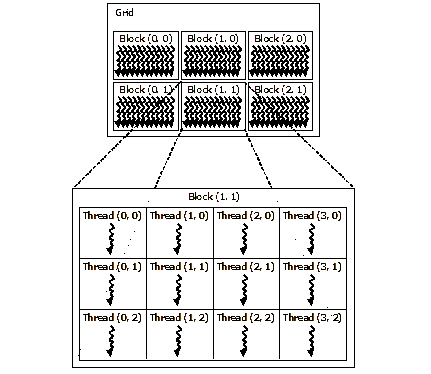
\includegraphics[width=0.65\linewidth]{cudaThreads.png}
    \caption{CUDA中的Thread、Block以及Grid}
    \label{fig:cudaThreads}
\end{figure}
\begin{figure}[htpb]
    \centering
    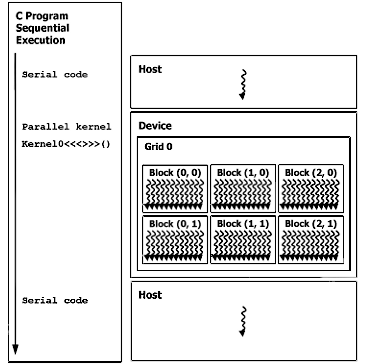
\includegraphics[width=0.65\linewidth]{cudaFlow.png}
    \caption{CUDA程序控制流}
    \label{fig:cudaFlow}
\end{figure}


\subsection{编写图像处理串行参照程序}
\label{sub:bian_xie_tu_xiang_chu_li_chuan_xing_can_zhao_cheng_xu_}
\par 在实际的编写并行的形态学图像处理程序之前,需要编写一个串行的图像处理算法,以用于作为功能上以及性能上的参照。
\par 首先,需要将磁盘中的图片读入内存。为了简便起见,使用cimg库读入图片。cimg\footnote{\url{http://cimg.eu/}}库是一个C语言的图像处理库,其只包含头文件,且性能较为优秀。图\ref{fig:grayScale}为使用cimg读入图片,然后进行灰度化后的结果。对于每一个点而言,计算其灰度(亮度)的公式如下(使用PAL制式):
\[ luminosity = 0.299\times red + 0.587\times green + 0.114\times blue \]
其中,\(red\)、\(green\)和\(blue\)分别为红、绿、蓝三个通道的亮度值,而\(luminosity\)则为所求灰度值。为了便于与其他程序进行对比,使用Lenna\footnote{\url{https://en.wikipedia.org/wiki/Lenna}}作为接下来所有图片处理程序的输入数据。
\par 为了能够对图片进行膨胀或蚀刻处理,首先需要将图片进行二值化处理。使用cimg中的\lstinline{threshold()}函数对于图像进行二值化,设置阈值为128,二值化的图形如图\ref{fig:binary}所示。需要注意,二值化的图片在内存中是使用0/1来表示的,而这一显示的图片还进行了在\([0, 255]\)区间上的归一化处理。

\begin{figure}[htpb]
    \centering
    \begin{minipage}{0.45\linewidth}
        \centering
        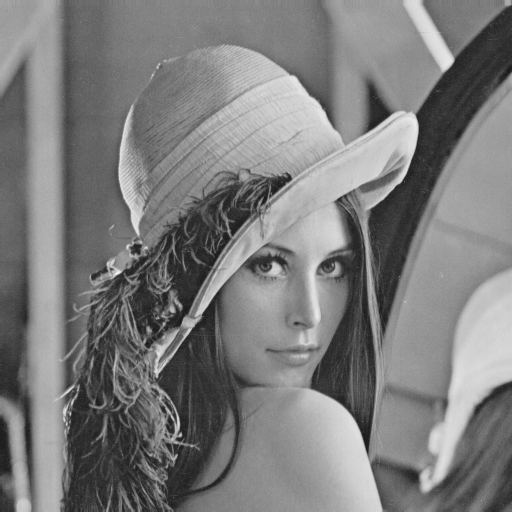
\includegraphics[width=0.9\linewidth]{grayScale.png}
        \caption{程序使用的样例图片(灰度化)}
        \label{fig:grayScale}
    \end{minipage}
    \hfill
    \begin{minipage}{0.45\linewidth}
        \centering
        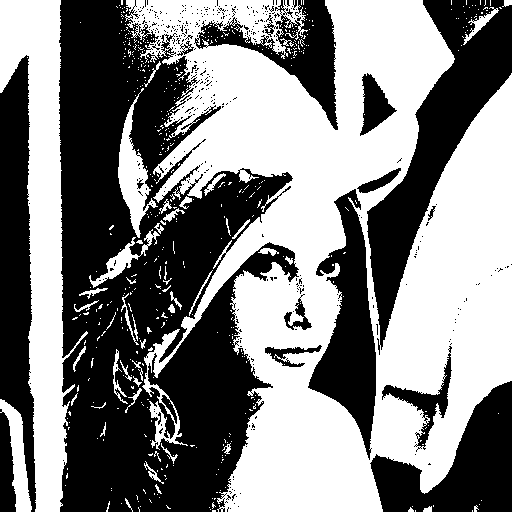
\includegraphics[width=0.9\linewidth]{binary.png}
        \caption{程序使用的样例图片(二值化)}
        \label{fig:binary}
    \end{minipage}
\end{figure}

\par 在上述预处理完成后,接下来对于图片进行蚀刻和膨胀处理。蚀刻和膨胀均采用\(5\times 5\)的kernel,其取值如下。kernel大小、形状和取值不同会导致膨胀或蚀刻的效果不同。
\[
    kernel_{\text{蚀刻}} =
    \begin{bmatrix}
        0 & 0 & 1 & 0 & 0 \\
        0 & 0 & 1 & 0 & 0 \\
        1 & 1 & 1 & 1 & 1 \\
        0 & 0 & 1 & 0 & 0 \\
        0 & 0 & 1 & 0 & 0
    \end{bmatrix}
    ,
    kernel_{\text{膨胀}} =
    \begin{bmatrix}
        1 & 1 & 1 & 1 & 1 \\
        1 & 1 & 1 & 1 & 1 \\
        1 & 1 & 1 & 1 & 1 \\
        1 & 1 & 1 & 1 & 1 \\
        1 & 1 & 1 & 1 & 1
    \end{bmatrix}
\]

\par 对于图片进行膨胀和蚀刻的串行算法如下:
\begin{simpleAlgorithm}{蚀刻和膨胀串行算法}
    \Procedure{ErodeAndDilate}{$image, kernel_e, kernel_d$}
    \For{each pixel $a$ \textbf{in} $image$}
        \State \(result_e\leftarrow 1, result_d\leftarrow 0\)
        \For{each pixel $b_e, b_d$ \textbf{in} $kernel_e, kernel_d$}
        \State find \(b_e\) or \(b_d\)'s corresponding pixel \(c\)
            \State \(result_e\leftarrow result_e\wedge (c\vee b_e), result_d\leftarrow result_d \vee (c\wedge b_d)\)
        \EndFor
        \State \(dilatedImage.at(a.pos)\leftarrow result_d, erodedImage.at(a.pos)\leftarrow result_e\)
        \EndFor
        \State \Return \(dilatedImage, erodedImage\)
    \EndProcedure
\end{simpleAlgorithm}
\par 可以看出,由于对于\(image\)的各个点之间的计算是没有依赖的,因此具有很强的可并行性。编写程序显示时刻和膨胀和膨胀后的图片,分别如图\ref{fig:eroded}和\ref{fig:dilated}所示。由于是对于白色的部分(二值图像中``1''的部分)进行蚀刻和膨胀,因此在腐蚀的图片中人像部分看起来变厚了,而在膨胀的图片中人像看起来变薄了。

\begin{figure}[htpb]
    \centering
    \begin{minipage}{0.45\linewidth}
        \centering
        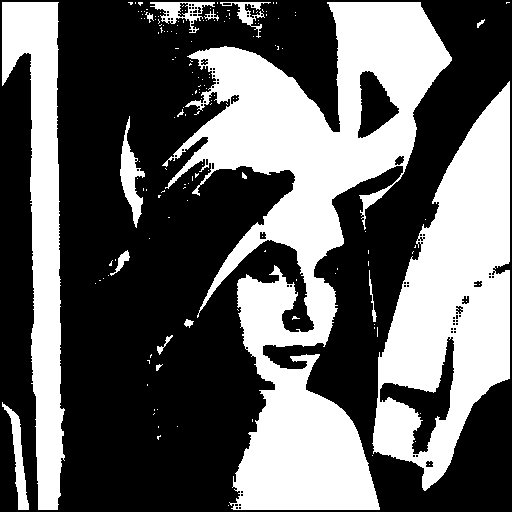
\includegraphics[width=0.9\linewidth]{eroded.png}
        \caption{蚀刻后的图片}
        \label{fig:eroded}
    \end{minipage}
    \hfill
    \begin{minipage}{0.45\linewidth}
        \centering
        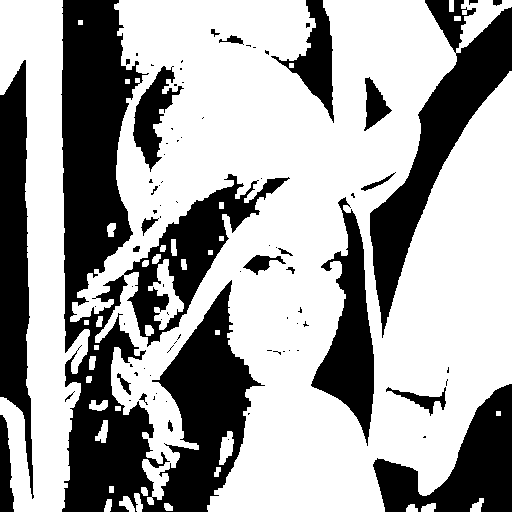
\includegraphics[width=0.9\linewidth]{dilated.png}
        \caption{膨胀后的图片}
        \label{fig:dilated}
    \end{minipage}
\end{figure}

\par 将蚀刻后的图片部分放大,可以看到反色的``十''字形状图案,如图\ref{fig:zoomed}所示,这是由于在蚀刻时使用了``十''字形的kernel导致的。如果kernel 取值不同,将产生不同形状的细节。
\begin{figure}[htpb]
    \centering
    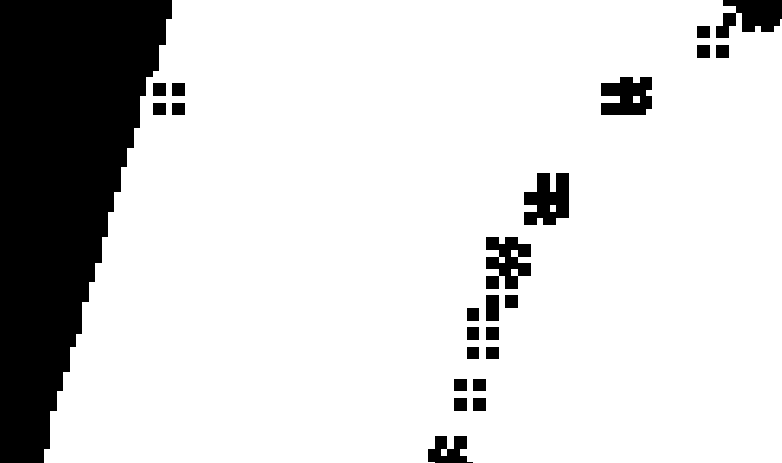
\includegraphics[width=0.3\linewidth]{zoomed.png}
    \caption{蚀刻后的图片(部分放大)}
    \label{fig:zoomed}
\end{figure}

\section{实验结果}
\par 通过这一阶段的调查和研究,以及对于各种并行方法的简单实践,并行编程的平台与环境已经准备充分。此外还有串行程序的结果作为参考。程序所示有的Lenna图片的大小为\(512\times 512\)由于处理一张图片的速度过快,无法进行性能的比较,因此在所有的程序中将图片处理的过程(仅蚀刻和膨胀的过程,不包含预处理)重复1000次,然后统计总时间以进行性能上的比较,这样可以减小各个并行平台初始化时间以及图片的预处理时间带来的影响。
\par 串行的程序在Intel\textsuperscript{\textregistered} Core\textsuperscript{\texttrademark} i7-7700K CPU @ 4.20GHz上运行,之后的并行程序也在此CPU上运行,以便于进行性能的比较。运行结果如图\ref{fig:lab1output}所示。

\begin{figure}[htpb]
    \centering
    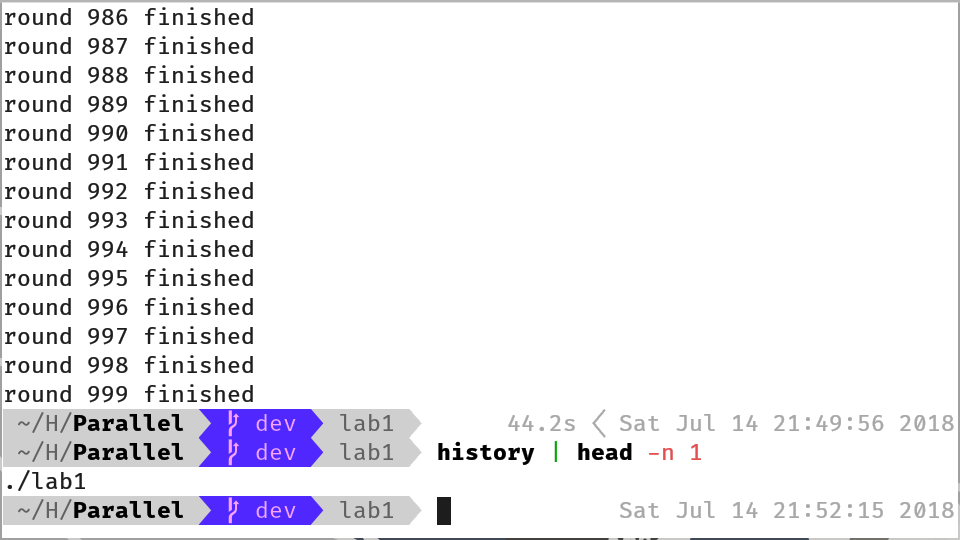
\includegraphics[width=0.9\linewidth]{lab1output.png}
    \caption{串行图像处理程序运行结果}
    \label{fig:lab1output}
\end{figure}

\par 从图中可以看出,程序运行的时间为44.2s,经过三次重复实验,平均时间也为44.2s,这将作为后续的时间比较基准。此处使用的是fish-shell插件omf的时间统计功能,统计的是一条命令执行的完整时间(walltime)。若需要在bash或zsh等其他shell内运行程序则需要自行编写统计时间的wrapper script。不使用程序内的时间统计是由于clock统计的为cpu时间,在执行并行程序时会将多个线程的时间相加,而在程序内直接统计walltime也可能由于程序的初始化步骤不同而不准确,因此直接在shell中统计时间才能较为完整的比较各个并行平台对于程序的优化能力。
\par 此外由于使用的是fish-shell,而fish-shell内建的history命令对于历史记录的排列与bash是相反的,因此在fish-shell中显示上一条命令的命令为history | head -n 1,在bash中等价的命令应为history | tail -n 1。


